% 17-16(본책 17쪽) — 가로 6칸·세로 4칸 도로망(A 왼쪽 위 · B 오른쪽 아래 · P 는 오른쪽 2칸·아래 2칸 · Q 는 오른쪽 4칸·아래 3칸 지점). 스캔 그림을 TikZ 로 다시 그림(스캔 화질).
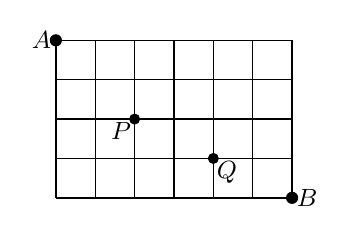
\begin{tikzpicture}[line width=0.5pt]
  \foreach \x in {0, 0.5, 1, 1.5, 2, 2.5, 3} { \draw (\x,0) -- (\x,2); }
  \foreach \y in {0, 0.5, 1, 1.5, 2} { \draw (0,\y) -- (3,\y); }
  \fill (0,2) circle (2.2pt);
  \node[left, font=\small, inner sep=1.5pt] at (0,2) {$\pt{A}$};
  \fill (3,0) circle (2.2pt);
  \node[right, font=\small, inner sep=1.5pt] at (3,0) {$\pt{B}$};
  \fill (1,1) circle (2pt);
  \node[below left, font=\small, inner sep=1pt] at (1,1) {$\pt{P}$};
  \fill (2,0.5) circle (2pt);
  \node[below right, font=\small, inner sep=1pt] at (2,0.5) {$\pt{Q}$};
\end{tikzpicture}
